\documentclass[9pt]{article}
\usepackage[utf8]{inputenc}
\usepackage{amsmath,amsthm,amsfonts,amssymb,amscd}
\usepackage{multirow,booktabs}
\usepackage{enumitem}
\usepackage{fancyhdr}
\usepackage{mathrsfs}
\usepackage{wrapfig}
\usepackage{setspace}
\usepackage{calc}
\usepackage{subfig}
\usepackage{multicol}
\usepackage{cancel}
\usepackage[retainorgcmds]{IEEEtrantools}
\usepackage{framed}
\usepackage[most]{tcolorbox}
\usepackage{tikz}
\usepackage{geometry}
\geometry{
	a4paper,
	total={170mm,257mm},
	left=20mm,
	top=20mm,
}
\title{Electrostatics}
\author{Aaron G.K.}

\begin{document}
	\maketitle
	\begin{center}
		\section*{Charges \& Fields}	
	\end{center}
	Electromagnetism is a broad field of physics which studies about electromagnetic interaction and it also happens to be one of the four fundamental forces in nature. A subfield is electrostatics which is the study of charges at rest. Electrostatics is manifested in various walks of life and has been studied throughout scientific history. \\ \\ For example, the Italian scientist Luigi Galvani (1737–1798) performed a series of experiments in which static electricity was used to stimulate contractions of leg muscles of dead frogs, an effect already known in humans subjected to static discharges. But Galvani also found that if he joined two metal wires (say copper and zinc) end to end and touched the other ends to muscles, he produced the same effect in frogs as static discharge. \\ \\ Alessandro Volta (1745–1827), partly inspired by Galvani’s work, experimented with various combinations of metals and developed the battery. During the same era, other scientists made progress in discovering fundamental connections. The periodic table was developed as the systematic properties of the elements were discovered. This influenced the development and refinement of the concept of atoms as the basis of matter. Such submicroscopic descriptions of matter also help explain a great deal more. Atomic and molecular interactions, such as the forces of friction, cohesion, and adhesion, are now known to be manifestations of the electromagnetic force. \\ \\ Static electricity is just one aspect of the electromagnetic force, which also includes moving electricity and magnetism. 	All the macroscopic forces that we experience directly, such as the sensations of touch and the tension in a rope, are due to the electromagnetic force, one of the four fundamental forces in nature. The gravitational force, another fundamental force, is actually sensed through the electromagnetic interaction of molecules, such as between those in our feet. (The other two fundamental forces, the strong nuclear force and the weak nuclear force, cannot be sensed on the human scale.)\\
	\subsection*{Static Electricity}
	Many of the characteristics of static electricity can be explored by rubbing things together. Static cling generated in the attraction of straw to recently polished amber also result from rubbing. Similarly, lightning results from air movements under certain weather conditions. You can also rub a balloon on your hair, and the static electricity created can then make the balloon cling to a wall. \\ \\
	\textbf{Characteristics of static electricity include}:
	\begin{itemize}
		\item The effects of static electricity are explained by a physical quantity not previously introduced, called electric charge.
		\item There are only two types of charge, one called positive and the other called negative.
		\item Like charges repel, whereas unlike charges attract.
		\item The force between charges decreases with distance.
	\end{itemize}
	Charges are usually carried by subatomic particles like protons and electrons. The charges of electrons and protons are identical in magnitude but opposite in sign. Furthermore, all charged objects in nature are integer-multiples of this basic quantity of charge, meaning that all charges are made of combinations of a basic unit of charge(elementary charge). Usually, charges are formed by combinations of electrons and protons. The magnitude of this elementary charge is
	$$\text{q}_\text{e}=1.60\times10^{-19}\text{C}$$ The symbol \textbf{q} is commonly used for charge and the subscript \textbf{e} indicates the charge of a single electron (or proton).
	The SI unit of charge is the coulomb (C). Since any charge in the universe is an integral multiple of the elementary charge, we have the following:
	$$\text{Q}=\text{nq}_\text{e}$$
	\subsection*{Law of Conservation of Charge}
	The total charge is constant in any process. \begin{center}
		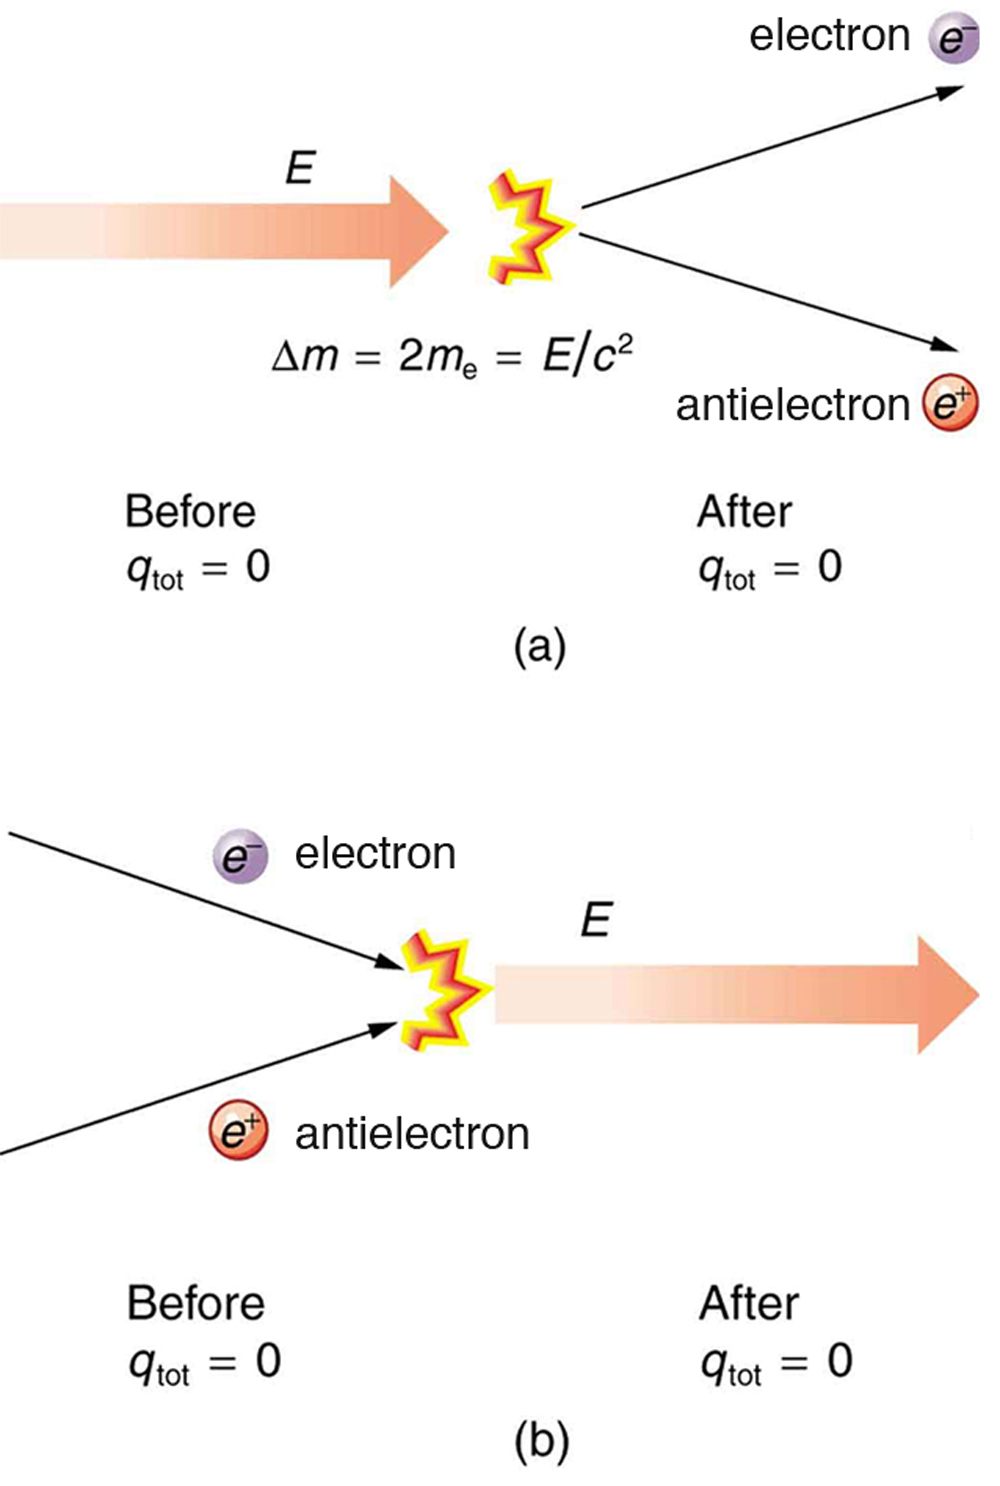
\includegraphics[scale=0.3]{charge_conservation.jpg}
	\end{center}
	In particle accelerators, mass can be created from energy. Sometimes, the created mass is charged, such as when an electron is created. Whenever a charged particle is created, another having an opposite charge is always created along with it, so that the total charge created is zero(because the net charge of a system is conserved). Usually, the two particles are “matter-antimatter” counterparts. For example, in the figure above: an antielectron would usually be created at the same time as an electron. The antielectron has a positive charge (it is called a positron), and so the total charge created is zero. Similarly, when an electron and a positron come together, they destroy each other and energy is formed from them.
	\subsection*{Charge Transfer} 
	Since charge is conserved, we can't create nor destroy it. However, we can transfer charges by various methods. Before we discuss those, let's review conductors \& insulators.  Some electrons in metals are not bound to individual atoms or sites in the material. These free electrons can move very freely. Any substance that has free electrons and allows charge to move relatively freely through it is called a conductor, materials that don't allow electrons to flow through them easily are called insulators. Here are some ways we can transfer charges:
	\subsubsection*{Conduction}
	 An electroscope is being charged by touching it with a positively charged glass rod in the figure below.
	 \begin{center}
	 	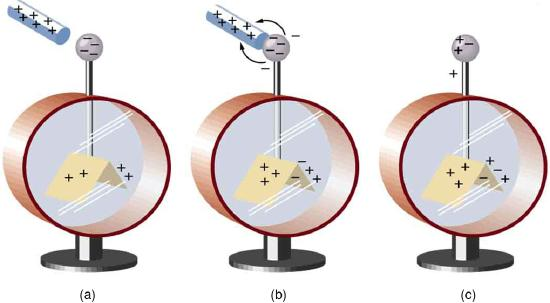
\includegraphics[scale=0.3]{electroscope}
	 \end{center} Because the glass rod is an insulator, it must actually touch the electroscope to transfer charge to or from it. Since only electrons move in metals, we see that they are attracted to the top of the electroscope. There, some are transferred to the positive rod by touch, leaving the electroscope with a net positive charge. Electrostatic repulsion in the leaves of the charged electroscope separates them. The electrostatic force has a horizontal component that results in the leaves moving apart. Similarly, the electroscope can be negatively charged by contact with a negatively charged object.
	\subsubsection*{Induction}	 
	Induction is best done with the induced polarization of neutral objects. Polarization is the separation of charges in an object that remains neutral. Look at the figure below for instance.
	\begin{center}
		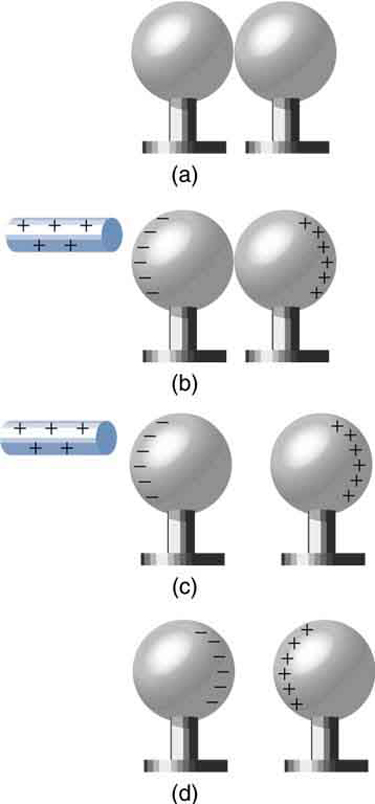
\includegraphics[scale=0.4]{induction}
	\end{center}If the spheres are now separated (before the rod is pulled away), each sphere will have a net charge. Note that the object closest to the charged rod receives an opposite charge when charged by induction. \\ \\
	Neutral objects(if they can be polarized) can be attracted to any charged object. The pieces of straw attracted to polished amber are neutral, for example. If you run a plastic comb through your hair, the charged comb can pick up neutral pieces of paper
	\subsection*{Cuolomb's Law}
	The mathematical formula for the electrostatic force is called Coulomb’s law after the French physicist Charles de Coulomb, who performed experiments and first proposed a formula to calculate it.
	\begin{quotation}
		Coulomb’s law calculates the magnitude of the force  F  between two point charges,  $\text{q}_1\text{  and  q}_2$ , separated by a distance r:
		$$\text{F}=\dfrac{\text{kq}_1\text{q}_2}{\text{r}^2}$$
		Where k is a constant which has a value of $\text{k}=\dfrac{1}{4\pi\epsilon_0}=8.99\times10^{9}\text{Nm}^2/\text{C}^2$
	\end{quotation}
	\subsection*{Electric Field}
	We have seen various types of forces so far. Most forces we experience daily are forces manifested through contact, but forces like the Cuolomb Force and gravity happen at a distance and don't necessarily need contact to be experienced or felt. Such forces are exerted through force fields. A field is generally a region in space such that a force is experienced. It is a way of conceptualizing and mapping the force that surrounds any object and acts on another object at a distance without apparent physical connection. For example, a charged rubber comb attracts neutral bits of paper from a distance by the Coulomb force. It is very useful to think of an object being surrounded in space by a force field. The force field carries the force to another object (called a test object) some distance away.  \\ \\
	Similarly, the Coulomb force field surrounding any charge extends throughout space. Using Coulomb’s law,  $\text{F}=\dfrac{\text{kq}_1\text{q}_2}{\text{r}^2}$, its magnitude is given by the equation  $\text{F}=\dfrac{\text{kQq}}{\text{r}^2}$ , for a point charge (a particle having a charge Q) acting on a test charge  q at a distance r. Both the magnitude and direction of the Coulomb force field depend on  Q  and the test charge  q . \\ \\
	To simplify things, we would prefer to have a field that depends only on the source Q and not on the test charge q. The electric field is defined in such a manner that it represents only the charge creating it and is unique at every point in space. Specifically, the electric field E is defined to be the ratio of the Coulomb force to the test charge:
	$$\mathbf{E}=\dfrac{\mathbf{F}}{\text{q}},$$ where  \textbf{F}  is the electrostatic force exerted on a positive test charge q.  It is important to note that  \textbf{E}  and \textbf{F} act in the same direction. It is also assumed that q is so small that it does not alter the charge distribution created by the source charge Q. According to Coulomb’s law, the force Q exerts on a test charge q is $\text{F}=\dfrac{\text{kQq}}{\text{r}^2}$. Thus the magnitude of the electric field, E , for a point charge is: 
	$$E=|\dfrac{F}{q}|=k|\dfrac{qQ}{qr^{2}}|=k\dfrac{|Q|}{r^{2}}.$$
	$$E=k\dfrac{|Q|}{r^{2}}$$
	Thus, we can see that the electric field by the source charge is to depend only on the charge Q and the distance r.
	\subsubsection*{Representing Field}
	To represent electric fields or fields in general, we use electric field lines. The lines are useful in visualizing field strength and direction. The electric field lines are defined for positive test charges(conventionally), and thus they show the direction of the force by a source charge acting on a positive charge. With that in mind, if we construct field lines for positive \& negative source charges, we get the following: \\ \\
	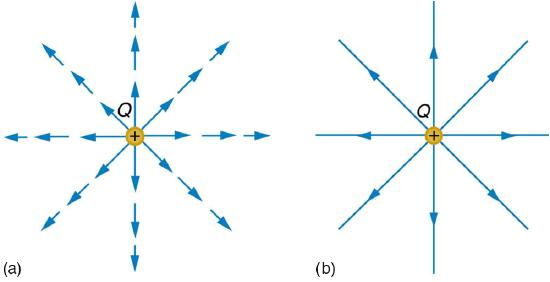
\includegraphics[scale=0.3]{source_p}\hspace{1in}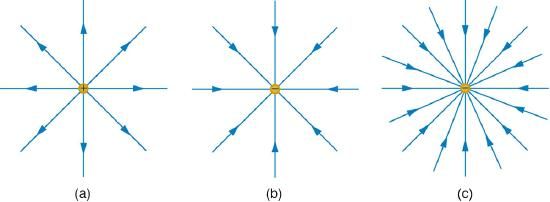
\includegraphics[scale=0.4]{source_n} \\
	On the left we have a positive source charge with an electric field around it while we have a negative source charge on the right. Although field lines are great tools, they are hypothetical. The properties of electric field lines for any charge distribution can be summarized as follows: \begin{itemize}
		\item Field lines must begin on positive charges and terminate on negative charges, or at infinity in the hypothetical case of isolated charges.
		\item The number of field lines leaving a positive charge or entering a negative charge is proportional to the magnitude of the charge.
		\item The strength of the field is proportional to the closeness of the field lines—more precisely, it is proportional to the number of lines per unit area perpendicular to the lines.
		\item The direction of the electric field is tangent to the field line at any point in space.
		\item Field lines can never cross.
	\end{itemize}
	
	
	
	
	
	
	
\end{document}	